% Two-sided document
\documentclass[12pt, twoside]{ociamthesis}
\usepackage{helvet}
\usepackage{amssymb}
\usepackage[utf8]{inputenc}
\usepackage[T1]{polski}
\usepackage{url}
\usepackage[hidelinks]{hyperref}
\usepackage[table,xcdraw]{xcolor}
\usepackage[leftbars]{changebar}
\usepackage{caption}
\hypersetup{
	pdftitle={Detekcja choroby Alzheimera i~stadium demencji z~użyciem narzędzi uczenia maszynowego w środowisku .NET},
	pdfsubject={Praca magisterska},
	pdfauthor={Mateusz Piotr Moruś},
	pdfkeywords={Choroba Alzheimera, demencja, uczenie maszynowe, uczenie transferowe, głębokie sieci neuronowe, sieci konwolucyjne, .NET, dotnet, CSharp, ML.NET, TensorFlow.NET}
}
\usepackage{graphicx}
\usepackage{listings}
\usepackage{xcolor}

\definecolor{codegreen}{rgb}{0,0.6,0}
\definecolor{codegray}{rgb}{0.5,0.5,0.5}
\definecolor{backcolour}{rgb}{0.95,0.95,0.92}

\lstdefinestyle{mystyle}{
    backgroundcolor=\color{backcolour},
    commentstyle=\color{codegreen},
    keywordstyle=\color{magenta},
    numberstyle=\tiny\color{codegray},
    stringstyle=\color{codegreen},
    basicstyle=\ttfamily\footnotesize,
    breakatwhitespace=false,
    breaklines=true,
    captionpos=b,
    keepspaces=true,
    numbers=left,
    numbersep=5pt,
    showspaces=false,
    showstringspaces=false,
    showtabs=false,
    tabsize=4
}

\lstset{style=mystyle}


\setlength{\changebarsep}{-5em}

\graphicspath{ {./Images/} }

\captionsetup[figure]{font=small}

% Make the numbering of figures continuous
\counterwithout{figure}{chapter}
% Make the numbering of tables continuous
\counterwithout{table}{chapter}

\title{Detekcja choroby Alzheimera i~stadium demencji z~użyciem narzędzi uczenia maszynowego w~środowisku .NET}
\engtitle{Detection of Alzheimer's disease and the stage of dementia using machine learning tools in the .NET environment}
\author{Mateusz Piotr Moruś}
\albumnumber{292540}
\university{UNIWERSYTET MARII CURIE-SKŁODOWSKIEJ W~LUBLINIE}
\college{Wydział Matematyki, Fizyki i~Informatyki}
\field{Informatyka}
\speciality{Deweloperska (programistyczna)}
\submittedtext{Praca magisterska}
\department{Katedrze Neuroinformatyki i~Inżynierii Biomedycznej}
\promoter{dr. hab. Grzegorza Marcina Wójcika, prof. UMCS}
\degreedate{Lublin rok 2023}

\begin{document}

% This baselineskip gives sufficient line spacing for an examiner to easily markup the thesis with comments
\baselineskip=18pt plus1pt

% Set the number of sectioning levels that get number and appear in the contents
\setcounter{secnumdepth}{3}
\setcounter{tocdepth}{3}

% Add a title page
\maketitle
% Insert a blank page after the title page
\cleardoublepage


\begin{abstract}

  Choroba Alzheimera jest najbardziej powszechną chorobą neurodegeneracyjną dotykającą współczesne społeczeństwo.
  Jej skutki a~także skutki szerszej pojęciowo demencji są również bardzo dotkliwe i~szczególne w~sposobie, w~jaki dotykają zarówno chorych jak i~ich bliskich.
  W~celu rozwoju perspektyw wczesnego wykrywania choroby w~niniejszej pracy przedstawiam możliwości wykorzystania metod uczenia maszynowego do detekcji choroby Alzheimera oraz stopnia demencji jej towarzyszącej.
  Wykorzystuję w~tym celu narzędzia uczenia maszynowego dostępne w~środowisku \emph{.NET}, które zostało całkowicie pominięte przez środowisko akademickie, natomiast jest bardzo popularne w~systemach medycznych czy szpitalnych, gdzie potencjalnie tego typu systemy diagnostyczne mogą być wykorzystywane.
  Porównuję dwa popularne narzędzia uczenia maszynowego -- bibliotekę \emph{ML.NET} oraz \emph{TensorFlow.NET}, które wykorzystuję w~celu przeprowadzenia uczenia transferowego oraz uczenia głębokich konwolucyjnych sieci neuronowych, które uczę i~testuję na zbiorze obrazów rezonansu magnetycznego mózgu osób zdrowych oraz z~chorobą Alzheimera i~o różnym stopniu demencji.
  Najlepszy wytrenowany model osiąga dokładność na poziomie $85\%$ dla klasyfikacji stopnia demencji, które nie jest wynikiem złym, choć alternatywne rozwiązania powstające w~ostatnich latach osiągają już znacznie lepsze wyniki.
  Przedstawiam także wady i~zalety wykorzystanych narzędzi oraz możliwości ich rozwoju w~przyszłości.

\end{abstract}

\begin{abstract-en}

  Alzheimer's disease is the most common neurodegenerative disease affecting modern society.
  On top of this, its effects and the effects of the wider concept of dementia are also very acute and particular in the way how they affect both patients and their loved ones.
  Aiming to push forward the prospects for early detection of the disease, in this thesis I~present the possibilities of using machine learning methods to detect Alzheimer's disease and the stages of dementia associated with it.
  For this purpose, I~use machine learning tools available in the \emph{.NET} environment, which has been completely neglected by the academic community, while it is very popular in medical or hospital systems, where potentially such diagnostic systems can be used.
  I~compare two popular machine learning tools -- the libraries called \emph{ML.NET} and \emph{TensorFlow.NET}.
  I~use them to perform transfer learning and using deep convolutional neural networks, I~carry out their training and test on a~dataset of brain MRI images of healthy subjects and those with Alzheimer's disease and varying stages of dementia.
  The best of the trained model achieves an accuracy of $85\%$ for classifying the stage of dementia, which is not a~bad result, although alternatives emerging in recent years are already performing much better.
  I~also present the advantages and disadvantages of the tools used and the potential for future development.

\end{abstract-en}


% Start roman page numbering
\begin{romanpages}
	% Generate and include a table of contents
	\tableofcontents
	% Create a group for list of figures and list of tables to fit both on one page
	\begingroup
	\let\clearpage\relax
	% Generate and include a list of figures
	\listoffigures
	% Generate and include a list of tables
	\listoftables
	\endgroup
% End roman page numbering
\end{romanpages}

\include{chapters/0-wstęp}
\chapter{Przegląd piśmiennictwa}

Choroba Alzheimera nadal nie jest w pełni zrozumiana, jednak dzięki badaniom zdobyto już wiele istotnych informacji na jej temat.
Część z nich opiera się wyłącznie na korelacjach i potwierdzonych powiązaniach z pominięciem przyczyn i konkretnych mechanizmów nimi rządzących, lecz nadal daje nam to wystarczający obraz by przedstawić kompleksowo opis choroby.

\section{Definicje i objawy choroby Alzheimera}

Definicje i objawy choroby Alzheimera.

\section{Diagnoza i stadium demencji}

Diagnoza i stadium demencji

\section{Metody tradycyjne detekcji choroby Alzheimera}

Metody tradycyjne detekcji choroby Alzheimera

\section{Narzędzia i techniki uczenia maszynowego}

Narzędzia i techniki uczenia maszynowego

\section{Istniejące podejścia do detekcji choroby Alzheimera z użyciem uczenia maszynowego}

Istniejące podejścia do detekcji choroby Alzheimera z użyciem uczenia maszynowego

\chapter{Metodologia i narzędzia uczenia maszynowego środowiska .NET}

Celem tej pracy jest wykorzystanie technologii uczenia maszynowego w środowisku .NET w celu detekcji choroby Alzheimera.
W tym rozdziale więc zostaną przedstawione narzędzia, które pomogą w osiągnięciu tego celu, w tym technologie uczenia maszynowego oraz sama platforma .NET.

\section{Technologie głębokiego uczenia maszynowego}

Teoretyczne zagadnienia związanie z technologiami głębokiego uczenia maszynowego, w szczególności głębokich konwolucyjnych sieci neuronowych zostały już omówione w sekcji \ref{sec:deep-learning}.
W tym rozdziale zostanie przedstawione w jaki sposób obiecująca teoria jest przekładana na wykorzystanie w praktyce.

\subsection{Symulator SNNS}

Tematykę oprogramowania służącego do tworzenia i trenowania sieci neuronowych warto zacząć omówienia przestarzałego już programu \emph{SNNS} (ang. Stuttgart Neural Network Simulator).
Pozwala on na tworzenie i trenowanie sieci neuronowych, a także -- co ważne przy jego zastosowaniach -- na ich wizualizację.

SNNS to program okienkowy napisany w języku C, przeznaczony głównie dla systemów Unixowych.
W ramach jego działania można zamodelować sieć neuronową po jednym neuronie, łącząc je z dużą dozą swobody w dowolne struktury oraz parametryzując je w dowolny sposób.
Następnie można zdefiniować zbiór danych uczących, a także zbiór danych testowych, na których można przeprowadzić proces uczenia sieci.

Całe tworzenie sieci jest czynnością bardzo czasochłonną i złożoną ze względu na manualną naturę definiowania jej struktury.
Daje za to bardzo dużo możliwości modyfikacji, w tym zmianę na przykład funkcji aktywacji pojedynczego neuronu, zachowania się konkretnego połączenia oraz wielu innych właściwości, które posiadają wszystkie obiekty możliwe do edycji w programie.

Najważniejszą cechą SNNS jest wizualny sposób budowy sieci neuronowej oraz manualny proces jej konfiguracji.
Nie jest ona może wtedy wystarczająco wydajna do jakichkolwiek problemów, z którymi potrafią radzić sobie nowoczesne sieci neuronowe, ale pozwala na zrozumienie ich działania oraz nauczenie się podstawowych zasad ich budowy.
Dlatego też mimo, iż sam program jest już przestarzały i wycofany z użytku a sami jego autorzy polecają użycie nowoczesnych bibliotek uczenia maszynowego takich jak TensorFlow czy PyTorch \cite{snns}, to nadal jest bardzo często wykorzystywany w celach edukacyjnych.

Pomimo, iż znane są metody znacznie przyspieszające działanie i uczenie sieci neuronowych przez reprezentacje wag i aktywacji jako macierzy i wektorów i ich późniejsze mnożenie przy pomocy zrównoleglonych obliczeń na kartach graficznych i dedykowanych urządzeniach, to założenia podstaw działania sztucznych sieci neuronowych pozostają niezmienne i programy typu SNNS pozwalają na znacznie prostsze ich poznanie i zrozumienie.

\subsection{Azure Machine Learning Studio}

\emph{Microsoft Azure Machine Learning Studio} (w skrócie \emph{AML Studio}) to kompleksowa platforma, która wykorzystywana jest do implementacji i zarządzania procesami uczenia maszynowego.
AML Studio oferuje zaawansowane narzędzia do tworzenia, wdrażania oraz monitorowania modeli uczenia maszynowego, integrując różnorodne etapy tego procesu w jednym środowisku.

Jest to platforma oparta na chmurze i posiadająca interfejs graficzny w postaci intuicyjnej strony internetowej, na której modelowanie przetwarzania danych i procesu uczenia odbywa się przy użyciu przeciągania i upuszczania elementów blokowych oraz łączenia ich w odpowiedni sposób.
Pozwala na tworzenie tak zwanych \emph{eksperymentów}, które składają się z kolejnych kroków w analizie danych i tworzeniu modeli.
Dzięki temu możliwe jest systematyczne badanie różnych podejść i łatwe porównywanie ich wyników.
Graficzny sposób reprezentacji wykorzystanych modułów w eksperymencie a także przepływu danych między nimi pozwala na uproszczenie wyszukiwania potencjalnych błędów lub problemów pojawiających się w całym procesie.
Możliwe jest również analizowanie w czasie rzeczywistym działania modelu i analizę przez niego danych w całym eksperymencie.

Bardzo istotną cechą AML Studio jest fakt, że platforma integruje się z innymi usługami chmurowymi dostarczanymi przez Microsoft Azure, co umożliwia tworzenie spójnych rozwiązań opartych na chmurze.
Pozwala na dynamiczne wczytywanie danych z innych źródeł znajdujących się w chmurze, a także na wdrażanie modeli uczenia maszynowego w postaci usług sieci Web, które mogą być wykorzystywane przez inne aplikacje.

Wykorzystanie Azure Machine Learning Studio dzięki swoim cechom pozwala na szybki trening modelu uczenia maszynowego oraz jego wdrożenie bez konieczności pisania kodu czy głębszej znajomości tematyki uczenia maszynowego \cite{mukunthu2019practical}, w szczególności gdy z założenia wdrożony model ma działać w chmurze i integrować się z innymi systemami w niej obecnymi.
Jednak w zastosowaniach, które nie czerpią korzyści z połączenia z chmurą i dają swobodę czasową na własnoręczne zaimplementowanie modelu, wykorzystanie AML Studio może być nieopłacalne ze względu na koszty związane z jego wykorzystaniem w większych ilościach.
Warto wtedy rozważyć inne rozwiązania, które dają swobodę konstruowania i trenowania modelu od podstawi i dostrojenie go do bardziej złożonych zadań, maksymalizując tym samym osiągane możliwości i dokładność -- a są to zazwyczaj biblioteki uczenia maszynowego w językach programowania.

\subsection{Tensorflow i Keras}

Jedną z najpopularniejszych bibliotek uczenia maszynowego, która jest wykorzystywana do tworzenia i trenowania sieci neuronowych jest \emph{Tensorflow}.
Jest to otwartoźródłowa platforma do obliczeń numerycznych i implementacji modeli uczenia maszynowego.
Jego fundamentem jest reprezentacja danych w postaci tensorów, co umożliwia wykonywanie skomplikowanych operacji matematycznych na dużych zbiorach danych \cite{shukla2018machine}.

Tensorflow jest bilbioteką niskopoziomową napisaną głównie w języku C++ i implementującą często używane algorytmy uczenia maszynowego i sieci neuronowych i wystawiającą je jako interfejs programistyczny w językach wyższego poziomu takich jak Python czy JavaScript.
Napisany został pierwotnie przez zespół badawczy Google Brain.

Jednak ze względu swoje dążenie do umożliwienia jak największej elastyczności i kontroli nad procesem uczenia sieci neuronowych, Tensorflow w swojej czystej postaci wymaga od programisty dużo pracy i wiedzy, aby zaimplementować nawet najprostszy model sieci neuronowej.

W celu uproszczenia z korzystania z Tensorflow powstały ``frontendy'' dla różnych języków programowania pozwalające na wykorzystanie jego możliwości w bardziej przyjazny sposób.
Jednym z nich jest \emph{Keras}, który jest wysokopoziomowym interfejsem programistycznym dla Tensorflow w języku Python.
Jest to jeden z najpopularniejszych interfejsów programistycznych dla Tensorflow ze względu na swoją prostotę i intuicyjność.

Dla uproszczenia wystawia API sekwencyjne (ang. Sequential API), które przez wykorzystanie istniejących klas i ``sekwencyjne'' tworzenie obiektów symbolizujących określone rodzaje warstw ze zdefiniowanymi odpowiednio parametrami pozwala na proste w śledzeniu i zrozumieniu stworzenie struktury sieci neuronowych.
Operacje takie jak \emph{skompilowanie} (czyli utworzenie z definicji warstw sieci zoptymalizowanego do uruchomienia i uczenia wstępnego modelu) definicji modelu używając odpowiednich parametrów czy uruchomienie trenowania (ang. \emph{fit}) w odpowiedniej konfiguracji wykonuje się wywołaniem tylko  jednej metody.

Mimo swojej prostoty, Keras pozwala na również na podejścia bardziej eksperckie.
W nich oprócz definiowania sekwencyjnego struktury sieci można również tworzyć własne klasy reprezentujące niestandardowe warstwy lub całe bloki odpowiednio ustrukturyzowane i zparametryzowane.

Uczenie sieci neuronowej w Keras zachowuje również zbiór metryk, które pozwalają na prześledzenie postępów w procesie uczenia i wykorzystanie ich do analizy lub optymalizacji modelu albo całego schematu programu.

Sukces Tensorflow oraz Keras wynika głównie z połączenia ich wydajności, elastyczności i prostoty użycia, które w dużej mierze są zasługą również wykorzystanego języka programowania Python, najpopularniejszego do zastosowań w uczeniu maszynownym.
Jednak ze względu na to, że obie te biblioteki mają swoje źródła dostępne na bazie licencji Apache 2.0 w publicznie dostępnym repozytorium serwisu GitHub \cite{tensorflow}.
Pozwala to społeczności na własne próby rozszerzenia zasięgu platformy do innych języków programowania, na przykład jak zostanie opisane w rozdziale \ref{sec:tensorflownet} -- do języka C\#.

\section{Platforma .NET}

Platforma .NET

\section{Framework uczenia maszynowego ML.NET}

\subsection{ML.NET Model Builder}

\subsection{Ręczne tworzenie modelu z użyciem ML.NET}

\label{sec:tensorflownet}
\section{Biblioteka Tensorflow.NET}

Tensorflow.NET

\chapter{Uczenie modelu detekcji choroby Alzheimera oraz jego wykorzystanie}

W tej pracy chcę przedstawić możliwości wykorzystania bibliotek uczenia maszynowego w środowisku \emph{.NET} w celu uczenia oraz późniejszego wykorzystania modelu głębokiej sieci neuronowej do detekcji choroby Alzheimera oraz stopnia demencji na obrazach rezonansu magnetycznego mózgów pacjentów, a także postaram się je porównać między sobą oraz z istniejącymi rozwiązaniami także spoza środowiska \emph{.NET}.

\section{Zbiór danych}

Wykorzystany zbiór pochodzi z platformy Kaggle (udostępniony jest pod adresem \url{kaggle.com/datasets/tourist55/alzheimers-dataset-4-class-of-images}, zapewniony na podstawie licencji \emph{Open Data Commons Open Database License} (\emph{ODbL}) wersji $1.0$) \cite{kaggle-alzheimers-dataset}.
Jest wstępnie podzielony na zbiór treningowy oraz testowy w celu zapewnienia powtarzalności i porównywalności wyników uzyskanych z użyciem różnych narzędzi i z różnych źródeł.
Zawiera on zestaw obrazów uzyskanych z badań rezonansem magnetycznym (MRI), których celem jest analiza i diagnoza otępienia spowodowanego chorobą Alzheimera.
Obrazy te są dwuwymiarowym wycinkiem trójwymiarowego skanu rezonansu magnetycznego mózgu, który najlepiej obrazuje strukturę mózgu i potencjalne zmiany chorobowe.
Mają wymiary $208 \times 176$ pikseli -- wystarczająco duże, aby widoczne były nawet drobne detale ale na tyle małe, aby były możliwe do przetworzenia przez mniejsze sieci neuronowe a także umożliwiły ich znacznie szybsze szkolenie.

Zbiór danych składa się z czterech kategorii obrazów, zarówno w zbiorze treningowym, jak i testowym:

\begin{itemize}

  \item
        Brak demencji (\emph{Non Demented}) -- ta kategoria zawiera obrazy mózgów osób niebędących dotkniętymi demencją.
        W zbiorze treningowym znajduje się 2560 obrazów, a w zbiorze testowym 640 obrazów, co daje sumarycznie 3200 zdjęć z tej kategorii.

  \item
        Bardzo łagodna demencja (\emph{Very Mild Demented}) -- zbiór ten obejmuje obrazy osób z bardzo łagodnym stopniem demencji.
        W zbiorze treningowym znajduje się 1792 obrazy, a w zbiorze testowym 448 obrazów, co daje łącznie 2240 obrazów z tej kategorii.

  \item
        Łagodna demencja (\emph{Mild Demented}) -- ten zbiór zawiera obrazy mózgów pacjentów cierpiących na łagodne otępienie związanego z chorobą Alzheimera.
        W zbiorze treningowym znajduje się 717 obrazów, a w zbiorze testowym 179 obrazów, co daje łączną sumę 896 obrazów z tej kategorii.

  \item
        Umiarkowana demencja (\emph{Moderate Demented}) -- ta kategoria obejmuje obrazy mózgów pacjentów już z wyższym stopniem demencji związanym z chorobą Alzheimera.
        W zbiorze treningowym znajduje się 52 obrazy, a w zbiorze testowym 12 obrazów, co daje łącznie 64 obrazy z tej kategorii.

\end{itemize}

\begin{figure}[ht]
  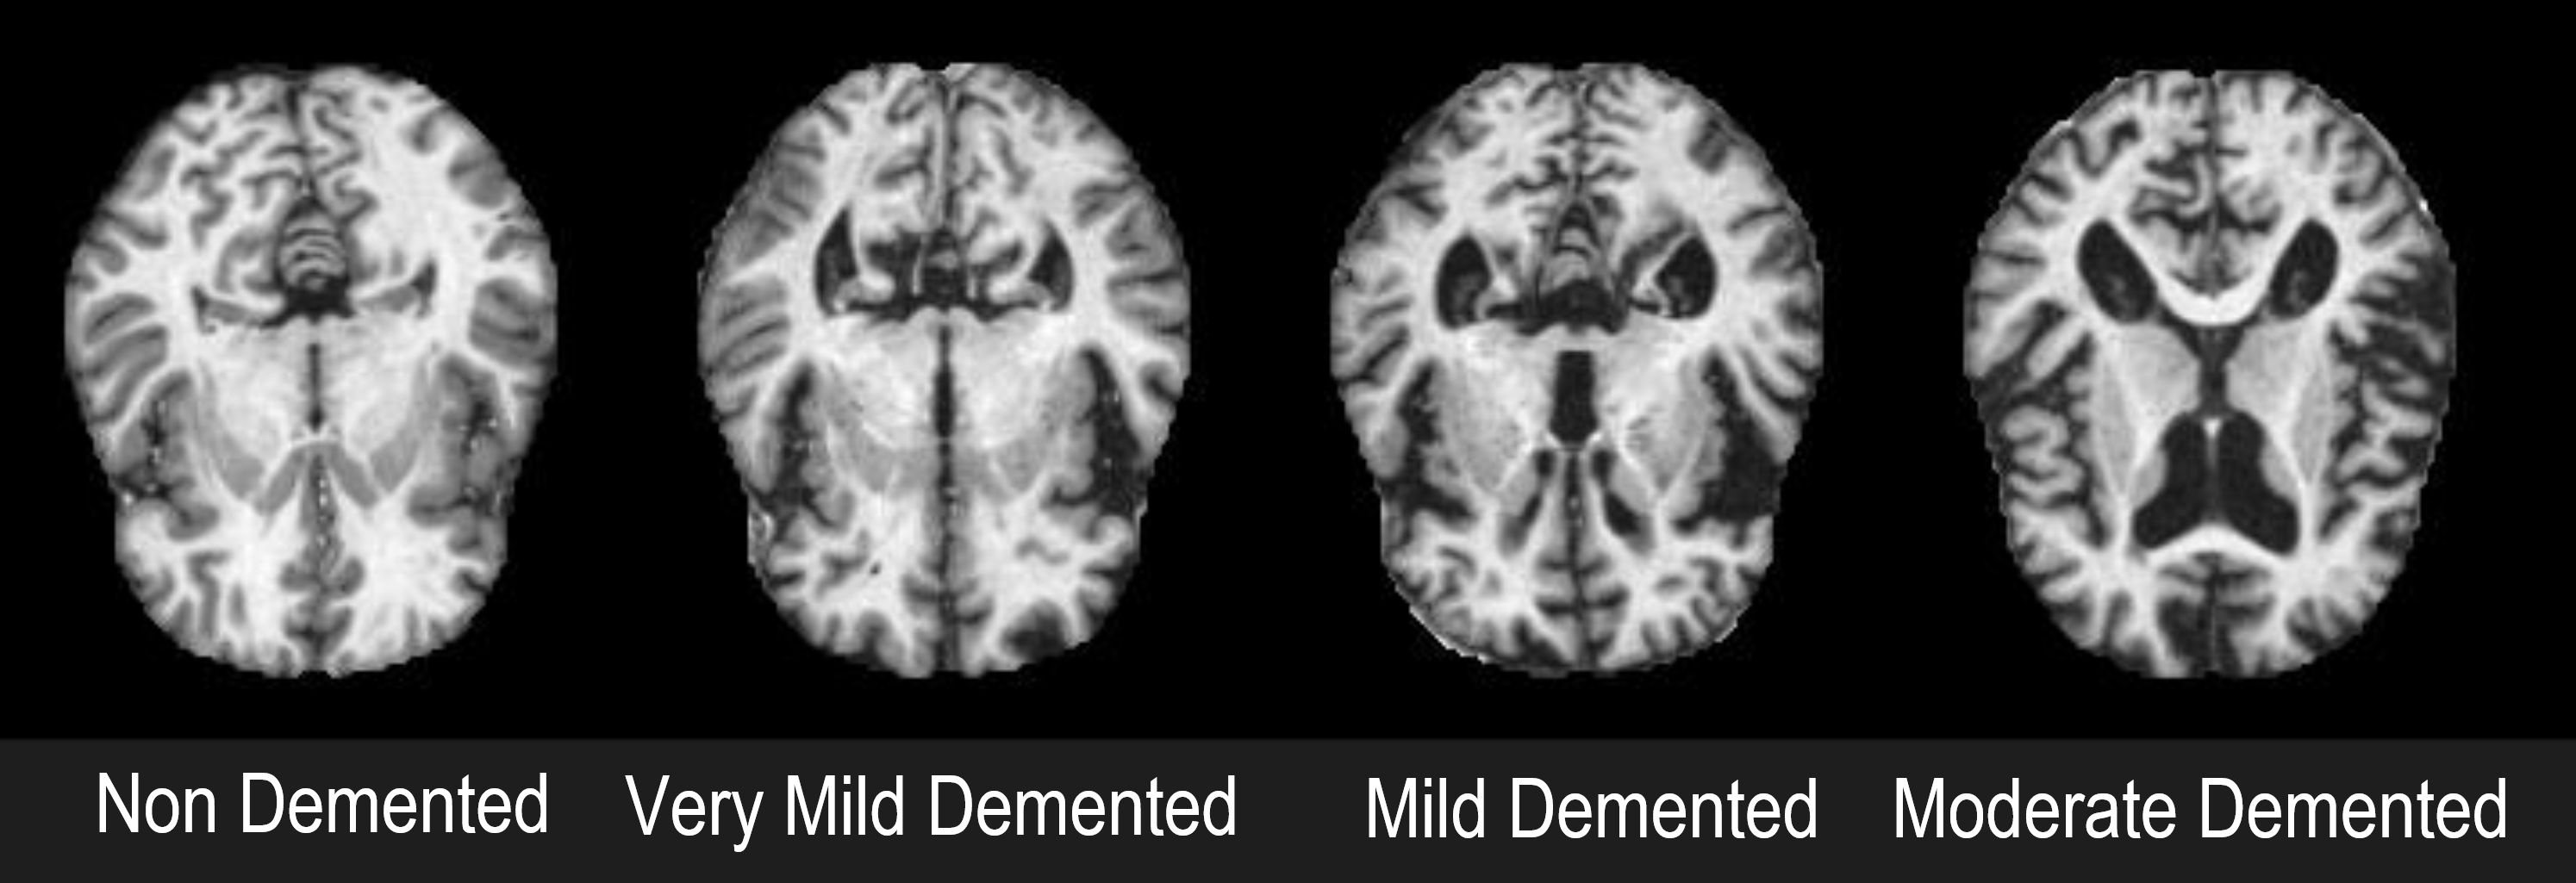
\includegraphics[width=\textwidth]{dataset-image-examples}
  \caption[Zestawienie przykładowych obrazów z każdej kategorii zbioru danych]{Zestawienie przykładowych obrazów z każdej kategorii zbioru danych \cite{kaggle-alzheimers-dataset}, gdzie przedstawione od lewej są: obraz mózgu osoby bez demencji, obraz mózgu osoby z bardzo lekką demencją, obraz mózgu osoby z lekką demencją o podłożach w chorobie Alzheimera oraz obraz mózgu osoby z umiarkowaną demencją chorą na Alzheimera.}
  \label{fig:dataset-image-examples}
\end{figure}

Przykłady obrazów z poszczególnych kategorii przedstawione są na \hyperref[fig:dataset-image-examples]{rysunku \ref*{fig:dataset-image-examples}}.

\section{Uczenie modelu z użyciem narzędzia ML.NET}

\subsection{Uczenie modelu z wykorzystaniem niestandardowego kodu biblioteki ML.NET}

\begin{figure}[ht]
  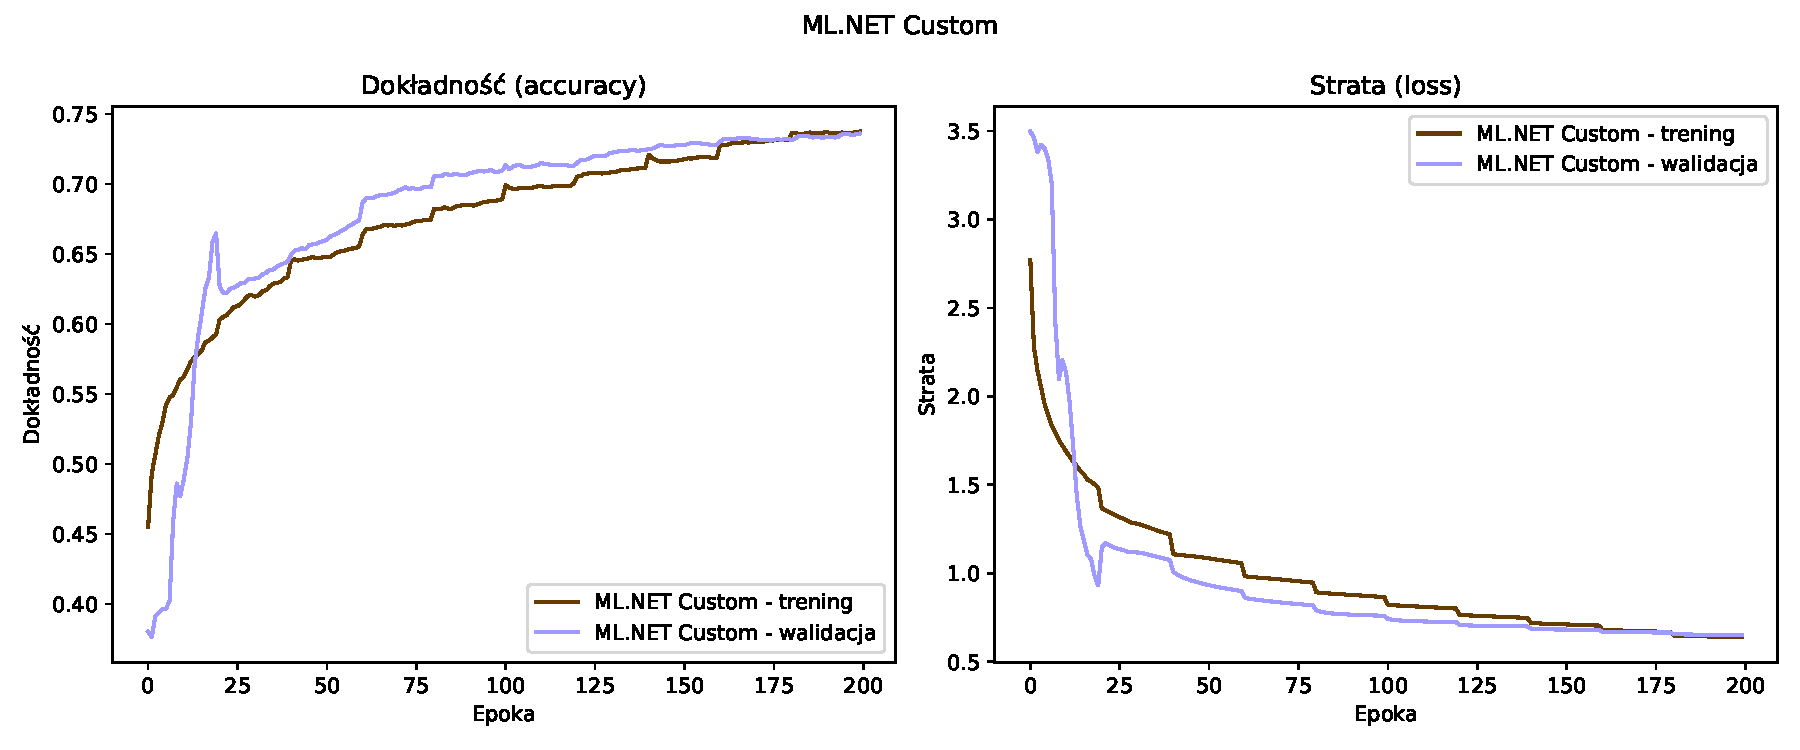
\includegraphics[width=\textwidth]{plot-mlnet-custom-training-overview}
  \caption[Wykresy statystyk modelu ML.NET Custom w trakcie uczenia]{Wykresy dokładności (\emph{accuracy}) oraz straty (\emph{loss}) dla danych testowych i walidacyjnych modelu ML.NET Custom w trakcie uczenia}
  \label{fig:plot-mlnet-custom-training-overview}
\end{figure}

\subsection{Uczenie modelu z użyciem narzędzia ML.NET Model Builder}

\begin{figure}[ht]
  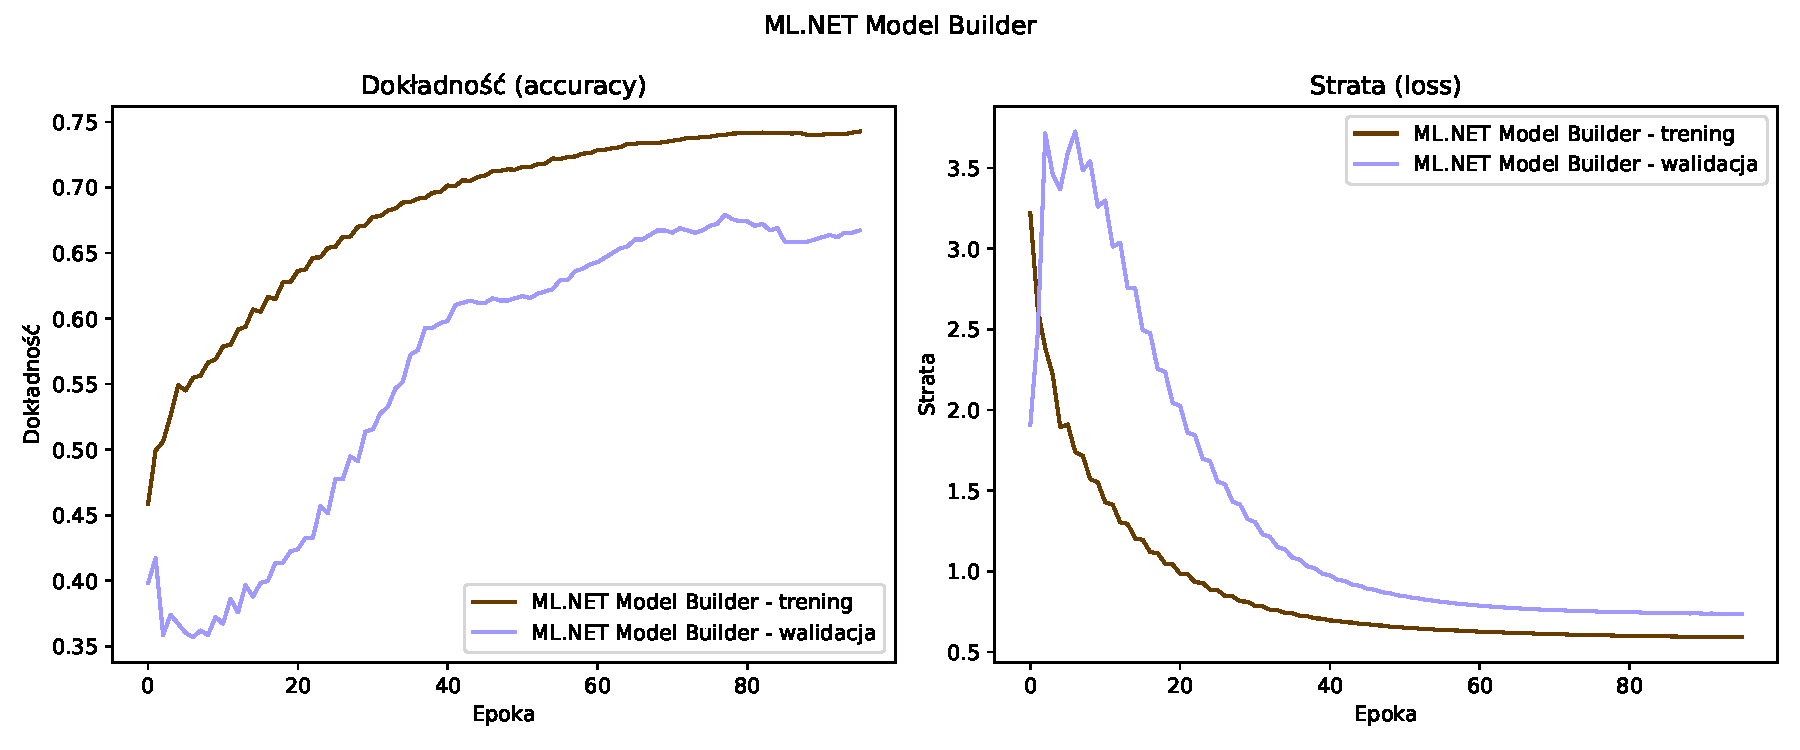
\includegraphics[width=\textwidth]{plot-mlnet-model-builder-training-overview}
  \caption[Wykresy statystyk modelu ML.NET Model Builder w trakcie uczenia]{Wykresy dokładności (\emph{accuracy}) oraz straty (\emph{loss}) dla danych testowych i walidacyjnych modelu ML.NET Model Builder w trakcie uczenia}
  \label{fig:plot-mlnet-model-builder-training-overview}
\end{figure}

\section{Uczenie niestandardowego modelu z użyciem biblioteki TenserFlow.NET}

\begin{figure}[ht]
  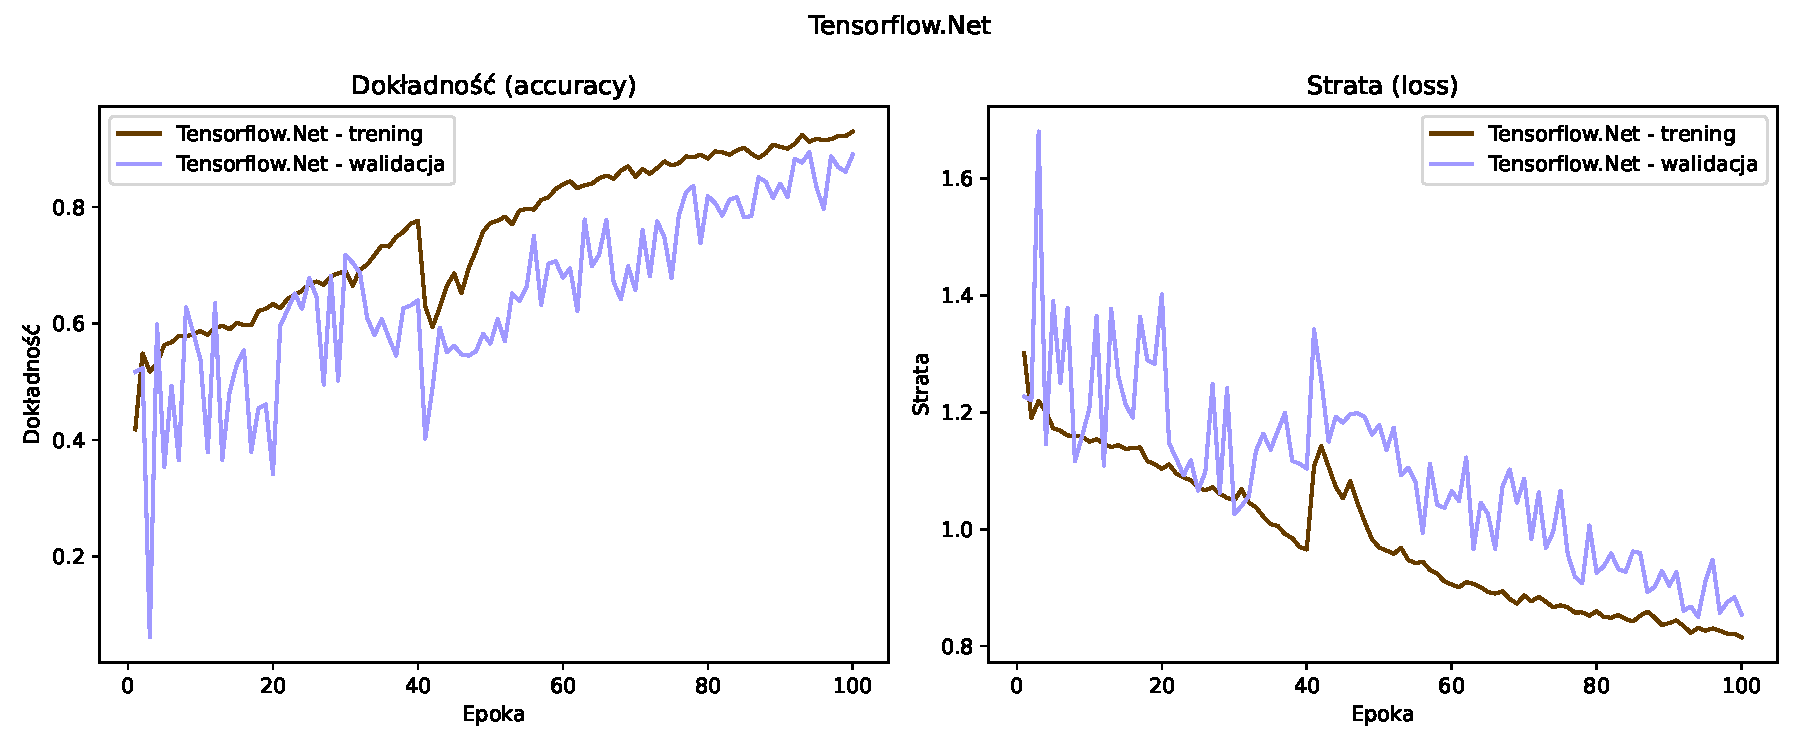
\includegraphics[width=\textwidth]{plot-tensorflownet-training-overview}
  \caption[Wykresy statystyk modelu Tensorflow.NET w trakcie uczenia]{Wykresy dokładności (\emph{accuracy}) oraz straty (\emph{loss}) dla danych testowych i walidacyjnych modelu Tensorflow.NET w trakcie uczenia}
  \label{fig:plot-tensorflownet-training-overview}
\end{figure}

Opis procesu uczenia modelu z użyciem biblioteki TenserFlow.NET

\section{Porównanie wyników}

\begin{figure}[ht]
  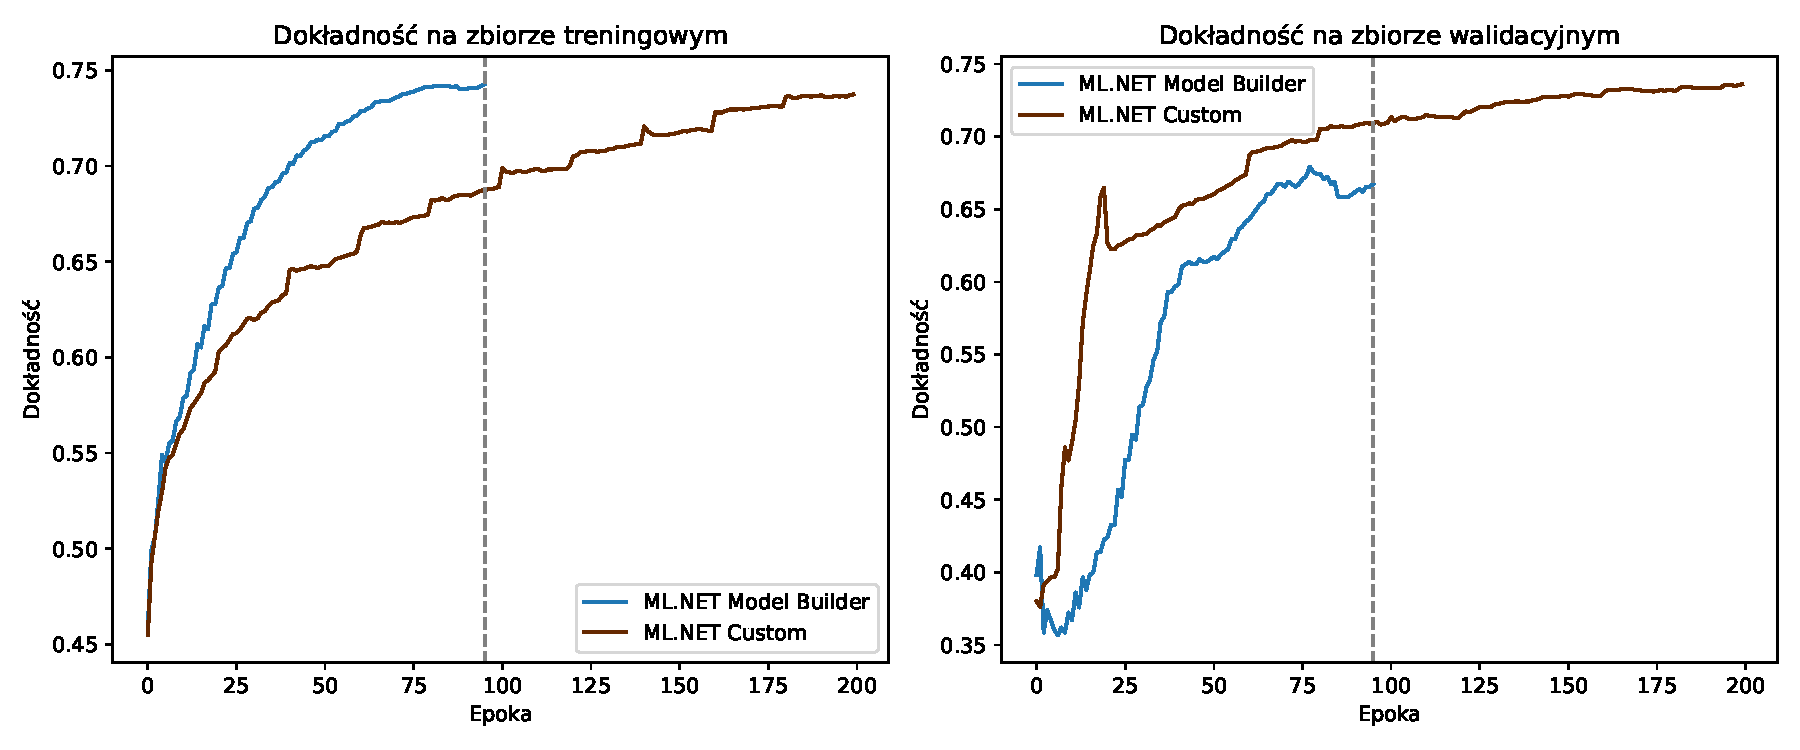
\includegraphics[width=\textwidth]{plot-mlnet-custom-vs-mlnet-model-builder}
  \caption[Porównanie dokładności oraz straty modeli ML.NET Custom oraz ML.NET Model Builder]{Porównanie dokładności (\emph{accuracy}) oraz straty (\emph{loss}) na zbiorze treningowym i walidacyjnym modeli z projektów ML.NET Custom oraz ML.NET Model Builder}
  \label{fig:plot-mlnet-custom-vs-mlnet-model-builder}
\end{figure}

\begin{figure}[ht]
  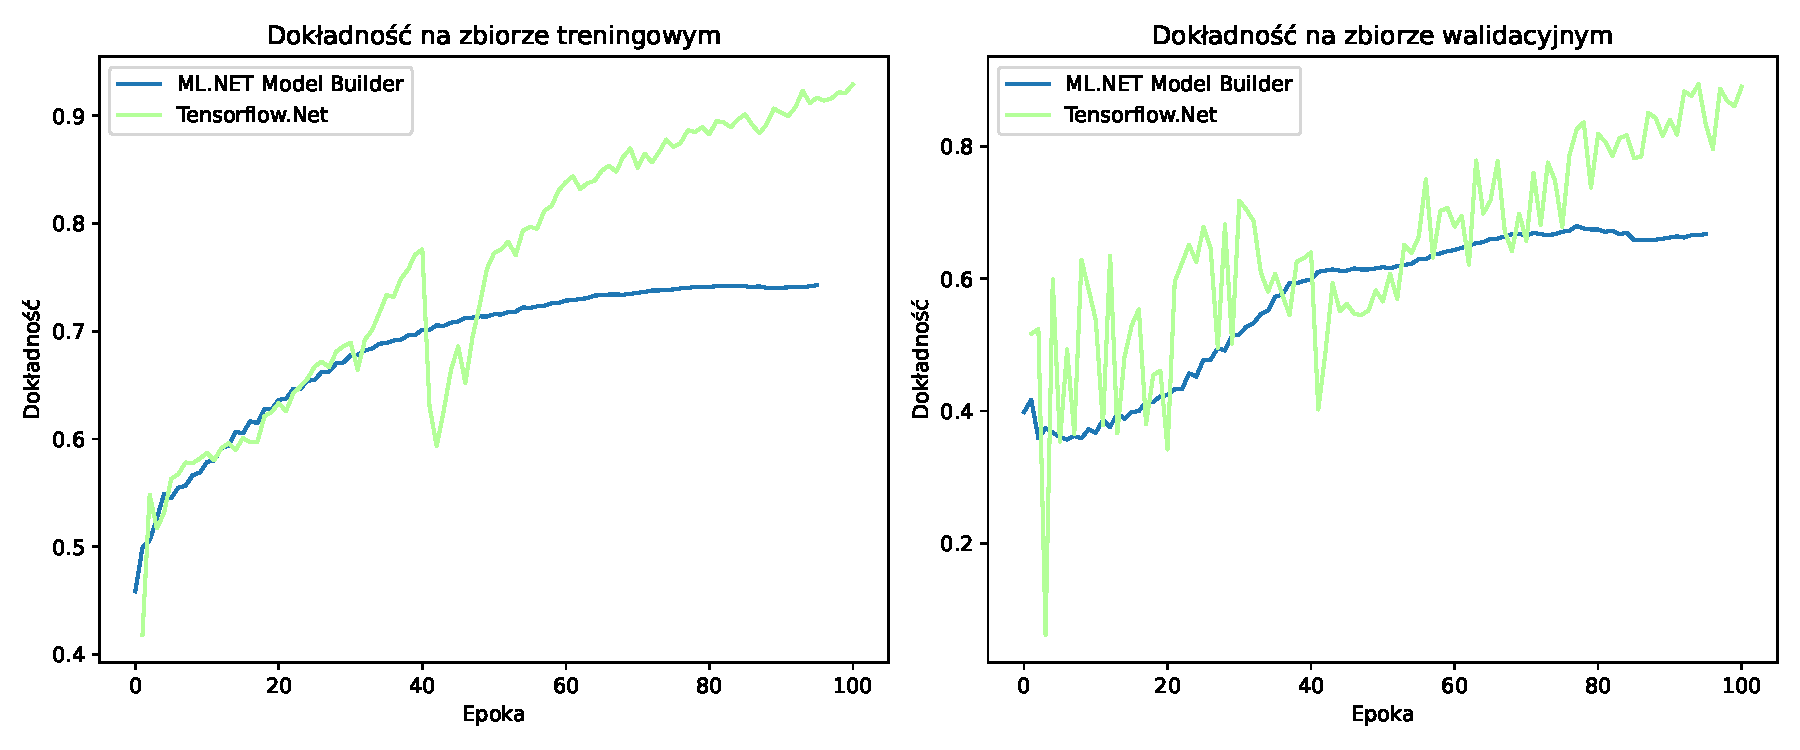
\includegraphics[width=\textwidth]{plot-mlnet-model-builder-vs-tensorflownet}
  \caption[Porównanie dokładności oraz straty modeli ML.NET Model Builder oraz Tensorflow.NET]{Porównanie dokładności (\emph{accuracy}) oraz straty (\emph{loss}) na zbiorze treningowym i walidacyjnym modeli z projektów ML.NET Model Builder oraz Tenserflow.NET}
  \label{fig:plot-mlnet-model-builder-vs-tensorflownet}
\end{figure}

\begin{table}[ht]
  \centering
  \begin{tabular}{|l|r|r|r|r|}
    \hline
                         & \multicolumn{2}{c|}{Zbiór treningowy}                                          & \multicolumn{2}{c|}{Zbiór walidacyjny}                      \\
    \cline{2-5}
                         & \multicolumn{1}{|c|}{Accuracy}        & \multicolumn{1}{|c|}{Loss}             & \multicolumn{1}{|c|}{Accuracy} & \multicolumn{1}{|c|}{Loss} \\
    \hline
    ML.NET Custom        & 0.7373874                             & 0.6378530                              & 0.7359702                      & 0.6511808                  \\
    ML.NET Model Builder & 0.7401715                             & 0.6036751                              & 0.6793103                      & 0.7503802                  \\
    Tensorflow.NET       & 0.9118868                             & 0.8311445                              & 0.8935547                      & 0.8501284                  \\
    \hline
  \end{tabular}
  \caption[Porównanie dokładności oraz straty modeli na zbiorze treningowym i walidacyjnym]{Porównanie dokładności (\emph{accuracy}) oraz straty (\emph{loss}) modeli na zbiorze treningowym i walidacyjnym w epokach szkolenia najlepszych względem na dokładności walidacyjnej}
  \label{tab:train_validation_metric_comparison}
\end{table}

\begin{table}[ht]
  \centering
  \begin{tabular}{|l|r|}
    \hline
                         & \multicolumn{1}{|c|}{Accuracy} \\
    \hline
    ML.NET Custom        & 0.45269742                     \\
    ML.NET Model Builder & 0.70602033                     \\
    Tensorflow.NET       & 0.85926505                     \\
    \hline
  \end{tabular}
  \caption[Porównanie dokładności modeli na tym samym zbiorze testowym]{Porównanie dokładności (\emph{accuracy}) modeli na tym samym zbiorze testowym}
  \label{tab:test_accuracy_comparison}
\end{table}

\section{Wykorzystanie modelu w aplikacji z użyciem biblioteki ML.NET}

W jaki sposób wykorzystać można model w aplikacji

\chapter{Dyskusja}

Dyskusja i porównanie z istniejącymi rozwiązaniami


% Add the Bibliography to the contents page
\addcontentsline{toc}{chapter}{Bibliografia}
% Use a bibtex bibliography file refs.bib
\bibliography{refs}
% Use the plain bibliography style ordered by citation
\bibliographystyle{unsrt}

\end{document}
